\chapter{归纳不变式自动生成工具的实现}\label{chap:implementation}

本章节将基于设计方案,详细介绍了归纳不变式自动生成工具的实现细节,包括模块之间的交互,以及模块的具体实现。

\section{候选不变式检验模块}

候选不变式检验模块主要的职责是对生成模块的生成的候选不变式的正确性,给出的候选归纳不变式的递归性,以及对新生成不变式的独立性进行判断。

候选不变式检验模块接入了TLC和Apalache,用户可以选择其一对生成的候选不变式进行验证。
TLC 和 Apalache 是两个常见的面向\TLA 规约的模型检查工具(model checker),可以使用相似的配置文件对规约进行验证,
但是,两者的结果输出格式不同,需要做分别处理。

由于Apalache需要用户对协议中的变量和常量做出类型的注释,因此,目前能够提供的测试集中大多数的规约都无法使用Apalache进行验证。
在系统实现时,我们默认状态下使用TLC作为系统的模型检查器。
当然,在条件允许时,用户可以设置系统的参数来使用Apalache作为系统的模型检查器。

在检验候选的不变式和归纳不变式时,如果出现反例,无论是对候选不变式的反例,还是对归纳不变式的归纳反例,都应该提取出来,返回给生成模块。

\subsection{model checker的配置文件和运行选项}

对于图\ref{fig:client_server}中的规约,TLC 和 Apalache 会使用默认的配置文件进行验证,
即以 $INIT$为初始状态,$NEXT$ 为状态转移关系,在状态变化的过程中验证 $Safe$ 安全属性的正确性。
用户也可以指定使用其他配置文件,以验证从不同状态出发和不同状态转移条件下的用户定义的不变式的成立与否。
比如说需要验证的不变式,可以放在$INVARIANT$ 字段下。
对于一些常量,用户也可以通过配置文件$CONSTANTS$字段进行定义。
一个典型的配置文件如下:
\begin{lstlisting}
INIT Init
NEXT Next

INVARIANTS Inv_0 Inv_1 Inv_2

CONSTANTS
...
\end{lstlisting}
我们可以简单的理解为,模型检测器可以判断$INIT \wedge NEXT \vDash INVARIANT$ 是否成立。
在不成立时,模型检测器会给出一个状态的链接,展示系统状态如何从初始状态转移到不满足不变式的状态。

我们希望TLC和Apalache为我们验证生成模块生成的候选不变式的正确性,独立性和与已有不变式析取结果的递归性。
在验证过程中,我们希望模型检查器能够输出验证结果,以及验证过程中的反例(Counterexample)。

验证不变式的正确性是验证这三种性质中最为简单的。
只需要将需要验证的候选不变式放入$INVARIANT$字段中,然后运行模型检查器即可。
如果没有报错,说明候选不变式在规约的有限实例上保持布尔值为真。

由于候选的归纳不变式是由一系列引理不变式和安全属性析取而来,且每一个析取子式都满足$Init \wedge Next \vDash Lemma$,
所以候选归纳不变式自然满足引理\ref{con:init}和\ref{con:safety}。
验证候选的归纳不变式的递归性质时,我们只需要验证引理\ref{con:inductive}的正确性,我们需要验证归纳不变式在状态转移后依然成立。
在此过程中,模型检查器弹出的报错就是归纳反例。

验证不变式的独立性是验证这三种性质中最为困难的。
检查不变式的独立性就是检查新生成的引理不变式是否能杀死(eliminate)候选的归纳不变式的归纳反例。
借助TLC,我们将系统的初始状态设置为这些归纳反例的状态之一,也就是将$INIT$ 设置为这些归纳反例状态的析取。
然后看在这些状态下,哪些新生成的引理不变式不成立。不成立便能代表他们能够杀死对应的归纳反例。
在操作中,我们需要用变量记录下这些引理不变式的值。
使用TLC的\textbf{"-dump"}选项将每个状态下的变量值输出到文件中,然后解析这些文件,找到能够杀死归纳反例的引理不变式。
如果归纳反例太多,会导致TLC计算状态转移关系的时间过长,状态转移图过于复杂。
尽管可以通过\textbf{"-workers"}选项添加TLC调用的线程数量,但是也收效甚微。
因此将归纳反例分组,分别使用一个线程对每一组归纳反例进行验证,可以有效减少验证时间。

但是这种做法并不充分,还需要通过$IndCand \wedge Next \nvDash Lemma$的结果来确认新引理不变式的独立性。


我们需要将新生成的不变式放到一个新的文件中,并使用关键字\textbf{EXTENDS} 将原有规约中的定义引入。
这样,我们就可以在新的文件中使用原有规约中的定义,和引入生成模块生成的候选不变式。
由于新的\TLA 文件中有着相似的结构,在验证同一个性质时,配置文件是可以复用的。
所以我们在系统运行之初就定义好配置文件中的内容,并写入硬盘供TLC/Apalache使用。

在使用TLC验证时,我们还需要关注诸多选项。
\textbf{"-config"}是我多样化使用TLC和apalache的关键,通过这个选项,我们可以指定TLC和Apalache的配置文件,以检验不变式的不同性质。
\textbf{"-deadlock"}选项用于检查是否存在死锁状态,如果选择了这个选项,那么TLC就不会检验死锁。
由于我们的目的是检验不变式的一些性质,所以我们不需要检验死锁,并选择了这一选项。
\textbf{"-continue"}选项揭示了TLC在检测出错误后是否继续运行,为了得到更多的反例,我们需要使用这个选项。

\subsection{model checker 的调用和结果解析}
本项目的代码主要基于Python实现,然而不论是TLC还是Apalache,都是Java实现的模型检查器,且没有可以直接调用的Python接口。
因此,我们需要通过Python的subprocess库来调用Java程序,并通过解析Java程序的命令行输出结果来获取验证结果。
在验证不同性质的时候指定好不同的配置文件并调整好不用的运行参数。

对于结果的解析,主要是将TLC或Apalache的输出结果进行解析,去除无用的信息,将有用的信息交给生成模块,以便强化学习模块调整策略,提高生成的候选不变式的正确性。
TLC和Apalache尽管两者有着不同的输出格式,但是他们的功能其实是一致的,都是将出现不变式错误时的状态,以及前序状态,也就是错误轨迹(error trace)。
错误轨迹的每一个节点都是一个状态,表达的是在这个状态下,各个变量的值。
TLC会以析取范式的形式将各个变量的值表达出来,而Apalache默认使用的json文件格式,将各个变量的值以键值对的形式表达出来。
我们需要将这些信息解析出来,以便强化学习模块能够理解这些信息,调整生成的候选不变式。

不变式反例和归纳反例有着相似的作用,都是用于提示用户或者生成模块,哪些状态下,不变式或者归纳不变式不成立。

类CTI的信息如图\ref{fig:class_cti}。在模型检测器检测去不变式或者归纳不变式的错误时,
通过类CTI中的静态方法\textbf{parse\_cti},可以将错误轨迹提取出来,生成多个不同的cti对象。
\begin{figure}[h]
    \centering
    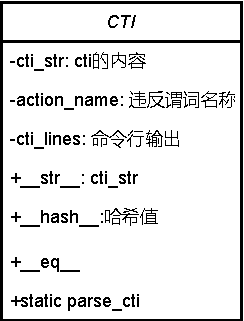
\includegraphics[width=0.3\textwidth]{figures/class_cti.pdf}
    \caption{CTI 类信息}
    \label{fig:class_cti}
\end{figure}
CTI类反应的是一个状态,在这个状态下,所有变量的值存储在\textit{cti\_str}字段中。
从这个状态出发,系统可以运行一个状态,这个状态下,给出的候选归纳不变式不成立。

CE类有着和CTI类相似的结构,不同的是,CE类更关注那个个使得不变式不成立的状态。


\section{候选不变式生成模块}

生成模块是本项目的关键,它负责生成候选不变式,检验模块是为生成模块服务的。
不同于以往的归纳不变式生成工具,使用随机枚举的方式生成候选不变式,我们引入强化学习来提高我们枚举的效率和成功率。
强化学习是一种通过智能体和环境的交互,智能体通过观察环境的状态,采取行动,获得奖励,来学习如何在环境中获取最大的奖励。
如图\ref{fig:rl}所示,一个强化学习模块可以分为智能体和环境两个部分。

\subsection{强化学习环境实现}

环境接收智能体的行动,做出反应并返回自身的状态和奖励,智能体根据环境的状态和奖励,调整滋生的策略,做出行动的选择。
本文使用\href{https://gymnasium.farama.org/}{gymnasium} \cite{gymnasium} 实现强化学习的环境。
gymnasium是一个开源的强化学习环境,提供了标准的环境接口,方便用户实现自己的强化学习环境,为我们实现环境提供了诸多便利。

自定义一个基于 gymnasium 的环境,最重要的是定义好环境的 \textbf{action\_space} 和 \textbf{observation\_space},以及实现step 函数。

\textbf{action\_space} 和 \textbf{observation\_space} 的数据类型都基于gymnasium的Space类,这其中包括众多类型。
\textbf{action\_space} 代表智能体所能采取的行动的空间,我们这里选择了\textbf{MultiDiscrete},智能体选择的行动为一个等同如输入的 \textbf{predicates} 长的向量。
这个向量每个维度的值都只能是0, 1, 2。在后续,我们会给这个向量 -1,得到一个每个维度上只有-1, 0, 1的向量,这个向量代表了我们的候选不变式。
每个维度上的值代表着对应的谓词是否被选择,-1代表否定,0代表不确定,1代表肯定。
向量与谓词相乘,便可以得到一个谓词表达式,再在前面加上定义好的量词,便可以得到一个候选不变式。

\textbf{observation\_space} 代表智能体所能观察到的环境的空间。
这里选择了\textbf{Dict} 类型。给予智能体参考的信息有:当前的不变式,对于当前不变式的反例或者归纳反例,可以选择的谓词,已经加入归纳不变式的不变式。
\textbf{Dict} 中每个键所对应的值也必须是一个Space类型,对于这四条信息,都选择了\textbf{Text}类型,也就是对应于字符串。

\textbf{step} 函数是环境的核心,它接受智能体的行动,返回环境的观察值,奖励和是否终止。
在我们的环境中,智能体的行动是一个向量,我们需要将这个向量转化为一个候选不变式,然后交给检验模块进行验证。
如果得到了归纳不变式,会给予100的奖励并退出。除此以外的所有情况,因为没有得到归纳不变式,所以都不会推出。
如果得到一个合适的不变式,会给予10的奖励,如果得到了一个错误的不变式,会给予-10的奖励。
如果得到一个不变式,但是不“独立”,会给予2的奖励,但是如果智能体简单地将正确的不变式合取上一个新的谓词,会给予-2的奖励。
与此同时,\textbf{step} 函数还需要返回观察值,这对应于observation\_space中的四条信息的数据结构。
这里复用了反例字段,在得到合适不变式时,返回归纳反例,否则,返回的是智能体提供的不变式的反例。
% 配个图
\begin{table}[!h]
    \label{table:award_punish}
	\centering
	\caption{奖励与惩罚的情况设置}
	\label{tab::situation}
	\renewcommand\arraystretch{1.4}
	\begin{tabular}{p{0.25\textwidth}p{0.15\textwidth}p{0.5\textwidth}}
		\toprule
		\textbf{候选不变式结果}   & \textbf{奖惩值} \\ 
        \midrule
		简单重复已有不变式 & -10 \\
		非不变式      & 0   \\
		被已有不变式覆盖  & 2   \\
		归纳不变式子式   & 10 \\
        \bottomrule
	\end{tabular}
\end{table}

\subsection{强化学习智能体实现}

实现智能体并不困难,gymnasium 的环境接口可以对接诸多的强化学习智能体实现框架。
本文选择了OpenAI \href{https://github.com/openai/baselines}{baselines}\cite{baselines}来实现智能体部分。
baselines 包括多种强化学习算法。
本文尝试了多种算法,包括DQN,PPO,A2C等算法。

\section{非功能模块}

非功能模块包括日志功能,计时功能,报错信息等,这些功能伴随着系统每个行为,为开发人员和用户提供更多信息,方便调试和使用。